%; whizzy chapter
% -initex iniptex -latex platex -format platex -bibtex jbibtex -fmt fmt
% $B0J>e(B whizzytex $B$r;HMQ$9$k>l9g$N@_Dj!#(B

%     Kansai Debian Meeting resources
%     Copyright (C) 2007 Takaya Yamashita
%     Thank you for Tokyo Debian Meeting resources

%     This program is free software; you can redistribute it and/or modify
%     it under the terms of the GNU General Public License as published by
%     the Free Software Foundation; either version 2 of the License, or
%     (at your option) any later version.

%     This program is distributed in the hope that it will be useful,
%     but WITHOUT ANY WARRANTY; without even the implied warranty of
%     MERCHANTABILITY or FITNESS FOR A PARTICULAR PURPOSE.  See the
%     GNU General Public License for more details.

%     You should have received a copy of the GNU General Public License
%     along with this program; if not, write to the Free Software
%     Foundation, Inc., 51 Franklin St, Fifth Floor, Boston, MA  02110-1301 USA

%  preview (shell-command (concat "evince " (replace-regexp-in-string "tex$" "pdf"(buffer-file-name)) "&"))
% $B2hA|%U%!%$%k$r=hM}$9$k$?$a$K$O(Bebb$B$rMxMQ$7$F(Bboundingbox$B$r:n@.!#(B
%(shell-command "cd image200708; ebb *.png")

%%$B$3$3$+$i%X%C%@3+;O!#(B

\documentclass[mingoth,a4paper]{jsarticle}
\usepackage{kansaimonthlyreport}
\usepackage[dvips]{xy}
\usepackage{ulem}

% $BF|IU$rDj5A$9$k!"Kh7nJQ$o$j$^$9!#(B
\newcommand{\debmtgyear}{2018}
\newcommand{\debmtgdate}{25}
\newcommand{\debmtgmonth}{3}
\newcommand{\debmtgnumber}{133}

\def\fixme#1{{\color{red}{#1}}}

\begin{document}

\begin{titlepage}

% $BKh7nJQ99$9$kItJ,!"K\J8$NKvHx$b=$@5$9$k$3$H$r$o$9$l$:$K(B

 $BBh(B\debmtgnumber{}$B2s(B $B4X@>(B Debian $BJY6/2q;qNA(B

\vspace{2cm}

\begin{center}

\includegraphics{image200802/kansaidebianlogo.png}
\end{center}

\begin{flushright}
\hfill{}$B4X@>(B Debian $BJY6/2qC4Ev<T(B $B:4!9LZ!&ARI_!&$N$,$?!&$+$o$@!&$*$*$D$-(B \\
\hfill{}\debmtgyear{}$BG/(B\debmtgmonth{}$B7n(B\debmtgdate{}$BF|(B
\end{flushright}

\thispagestyle{empty}
\end{titlepage}

\dancersection{$B:G6a$N(BDebian$B4X78$N%$%Y%s%HJs9p(B}{Debian JP}

\subsection{$BBh(B132$B2s4X@>(BDebian$BJY6/2q(B}
2 $B7n(B 25 $BF|$KJ!Eg6hL1%;%s%?!<$G3+:E$5$l$^$7$?!#H/I=$O@>;3OB9-$5$s$K$h$k!V(Bufw $B:FF~Lg!W$G$7$?!#(B 

\subsection{$BBh(B161$B2sEl5~%(%j%"(BDebian$BJY6/2q(B}
3 $B7n(B 24 $BF|$K?7=I9B8}%/%j%K%C%/$G3+:E$5$l$^$7$?!#H/I=$O(B ysaito $B$5$s$K$h$k(B $B!V(Bgo/debian $B$G$N5!3#3X=,4D6-9=C[$K$D$$$F!W(B

\begin{itemize}
		\item $B8=:_!"5!3#3X=,$K$O(B R $B$d(B python $B$rMxMQ$9$k$3$H$,I8=`E*$JA*Br;h$G$9!#(B
		\item $BBh;0$NA*Br;h$H$7$F!"(Bgo $B$rMxMQ$7$?5!3#3X=,$N<BA)!"$*$h$S!"(Bdebian$B>e$G$N%G!<%?%P!<%8%g%K%s%0!"%Q%$%W%i%$%s9=C[$rNc<($7$^$9!#(B
		\item $B5!3#3X=,$N8DJL$N%"%k%4%j%:%`$K$OF'$_9~$^$:!"4D6-9=C[$K$D$$$F%]%$%s%H$r$*EA$($7$^$9!#(B
\end{itemize}

\dancersection{$B:G6a$N(BDebian News}{Debian JP}

\subsection{2018/Mar/10th Stretch 9.4 $B$,%j%j!<%9(B}
\subsection{2018/Mar/16th Debian Conference 2018 registration $B3+;O(B}
			call for parapers $B$O(B 2018/June/18th https://debconf18.debconf.org/cfp/

\dancersection{$B;vA02]Bj(B}{$B4X@>(BDebian$BJY6/2q(B}

$B:#2s$N;vA02]Bj$O$"$j$^$;$s$G$7$?!#(B

$B;22C<T$N3'$5$s$O0J2<$NDL$j$G$9(B:
$B;vA02]Bj$O$"$j$^$;$s$G$7$?!#(B

\begin{prework}{ ipv6waterstar }
\end{prework}

\begin{prework}{YukiharuYABUKI}
\end{prework}

\begin{prework}{ yosuke\_san }
\end{prework}

\begin{prework}{gdevmjc}
\end{prework}

\begin{prework}{sato\_makoto}
\end{prework}

\begin{prework}{nogajun}
\end{prework}

\begin{prework}{murase\_syuka}
\end{prework}

\begin{prework}{t3rkwd}
\end{prework}


\dancersection{$B2f$,2H$N2>A[%M%C%H%o!<%/(B}{$B@n9>!!9@(B}

\subsection{$B$O$8$a$K(B}
$B2f$,2H$N%5!<%P72$N2>A[%M%C%H%o!<%/$O!"%7%s%/%i%$%"%s%H$rA0Ds$K9=C[$7$F$$$^$9!#%7%s%/%i%$%"%s%H!J(Bthin client$B!K$H$OC<Kv$K:G>.8B$N=hM}$r$5$;!"$[$H$s$I$N=hM}$r%5!<%PB&$K=8Cf$5$;$?%7%9%F%`%"!<%-%F%/%A%cA4HL$N;v$G$9!#2f$,2H$G$O(Bqemu-kvm$B!"(Bqemu$B$r;H$C$F(BVM$B!J(BVirtual Machine $B0J2<(BVM$B!K$K3F<o%5!<%P$r%$%s%9%H!<%k$71?MQ$7$F$$$^$9!#(B

$B$?$@$7:,K\E*$JLdBj$H$7$F!"<B(BPC$B>e$G(Bqemu-kvm$B$d(Bqemu$B$r;H$C$FJ#?t$N(BVM$B$rAv$i$;$k;v$O%5!<%P!"%M%C%H%o!<%/$NIi2Y$rA}Bg$5$;!"(BVM$B<+BN$N%Q%U%)!<%^%s%9$bDc2<$5$;$^$9!#$^$?!"%G!<%?$N6&M-$d3hMQ$G$bLdBj$r@8$8$^$9!#$=$3$G!"5U@bE*$JJ}K!$G$9$,!"%m!<%+%k(BPC$BB&$G$b(BVM$B$rAv$i$;!"2>A[%M%C%H%o!<%/$r9=C[$9$k;v$G0J>e$NLdBj$r7Z8:$7$^$9!#(B

$B$^$?!"0J2<$N;EMM$O%Q!<%=%J%k%Y!<%9$G$N1?MQ$rA0Ds$K9=C[$7$?$b$N$G$9!#;EMM$r;n$=$&$H$9$k$H$-$O!"I,$:%G!<%?Ey$N%P%C%/%"%C%W$r$H$C$F<+8J@UG$$G9T$C$F2<$5$$!#$h$j>\$7$/CN$j$?$$J}$O@lLg$N=q@R$d%;%_%J!<$J$I$r;29M$K$7$F$/$@$5$$!#(B

\subsection{$B2>A[%M%C%H%o!<%/$N35MW(B}
$B2>A[%M%C%H%o!<%/$K$O!"30It@\B3MQ%5!<%P!"J#?t$N(BVM$B!"%m!<%+%k%M%C%H%o!<%/$N$_$K$D$J$,$C$F$$$kJ#?t$NC<Kv!J%?%V%l%C%HEy!K$,$"$j$^$9!#$3$l$i$N%^%7%s$K%5%V%M%C%H$G#3$D$N%V%m%C%/!J(B192.168.24.0/25 192.168.24.128/26 192.168.24.192/26$B!K$K!"J,3d$7$?%M%C%H%o!<%/$4$H$N%W%i%$%Y!<%H(BIP$B%"%I%l%9$r3d$jEv$F!"MxJX@-$r3NJ]$7$^$9!#6qBNE*$K$O(B
\begin{itemize}
\item $B30ItMQ%M%C%H%o!<%/(B\\
  $B30ItMQ%M%C%H%o!<%/$O%$%s%?!<%M%C%H$K$D$J$0$?$a!"(BPR-500MI$B!J(BNTT$B$N%k!<%?!K$r;H$$$^$9!#$3$N%k!<%?$OC<Kv!J<B5!!"(BVM$B$rLd$o$:!K$N%M%C%H%o!<%/%G%P%$%9$N(BMAC$B%"%I%l%9$r8x3+$9$k;v$G!"3:EvC<Kv$rD>@\%$%s%?!<%M%C%H$K$D$J$0;v$,$G$-$^$9!#(B\\
  $B$3$N%k!<%?$N5!G=$H(BDNS$B$H$7$F;H$&(Bbind$B%=%U%H%&%'%"$N3F%9%F!<%?%9$rMxMQ$7$F!"3F(BVM$B$4$H$K(B192.168.24.0/25$B%V%m%C%/$N%W%i%$%Y!<%H(BIP$B%"%I%l%9$r3d$jEv$F!"(B1$B$D$N%0%m!<%P%k%"%I%l%9$GJ#?t$N30It8x3+MQ(BVM$B$r1?MQ$7$^$9!#(B
\clearpage
\item $BFbItMQ%M%C%H%o!<%/(B\\
  $BFbItMQ%M%C%H%o!<%/$O4pK\E*$K(BWifi$B$G$N@\B3$rA0Ds$H$7$^$9!#$5$i$K!"<B5!$N%m!<%+%k(BPC$B<+BN$O;}$A1?$V$N$G%F%6%j%s%0$G$N@\B3$b$G$-$k$h$&$K$7$^$9!#(B\\
  $B$^$?!"<B:]$N:n6H$d%"%W%j%1!<%7%g%s$N3hMQ$O(BVM$B$G9T$&$N$G!"%m!<%+%k(BPC$B<+BN$K$O(B192.168.24.0/25$B$N%V%m%C%/$N(BIP$B%"%I%l%9$r!"%m!<%+%k(BPC$BFb$GAv$k(BVM$B$K$O99$K%5%V%M%C%H%^%9%/$G(B2$B$D$KJ,$1$?!"(B192.168.24.128/26$B$N%V%m%C%/$H(B192.168.24.192/26$B$N%V%m%C%/$N(BIP$B%"%I%l%9$r3d$jEv$F$^$9!#(B
\end{itemize}
$B3F%M%C%H%o!<%/$N@_Dj$O0J2<$NDL$j$G$9!#(B

\subsection{$B30ItMQ%M%C%H%o!<%/(B}
\subsubsection{$B30ItMQ%M%C%H%o!<%/$N35MW(B}
$B30ItMQ%M%C%H%o!<%/$O!"(BPR-500MI$B$G30It%M%C%H$K$D$J$,$j!"Bh0l5AE*$J%W%i%$%Y!<%H%M%C%H%o!<%/$N%;%0%a%s%H$r9=@.$7$^$9!#$3$N%;%0%a%s%H$G$O30It8x3+MQ$N3F<o%5!<%P!"F1%;%0%a%s%H$N$_%"%/%;%92DG=$J%U%!%$%k%5!<%P!"%?%V%l%C%H7?(BPC$B!"%b%P%$%k5!4o$J$I$,$"$j!"$3$l$i$r%$!<%5%M%C%H$d(BWifi$B$G@\B3$7$F$$$^$9!#(B

$B$^$?!"F1%;%0%a%s%H$K@\B3$7$F$$$k(BHand made$B$N(Brouter$B$O$5$i$K(B192.168.18.0/24$B$N%;%0%a%s%H$K$D$J$,$C$F$$$^$9!J$?$@$7!"8=:_$O(BSSH$B$r;H$C$F!"(BVM$B$N%[%9%H(BPC$B$rJ]<i$9$k$N$_!K!#6qBNE*$J%$%a!<%8$O2<?^$N$h$&$K$J$j$^$9!#(B

%$B?^7A$NA^F~(B
\begin{figure*}[!h]
\centering
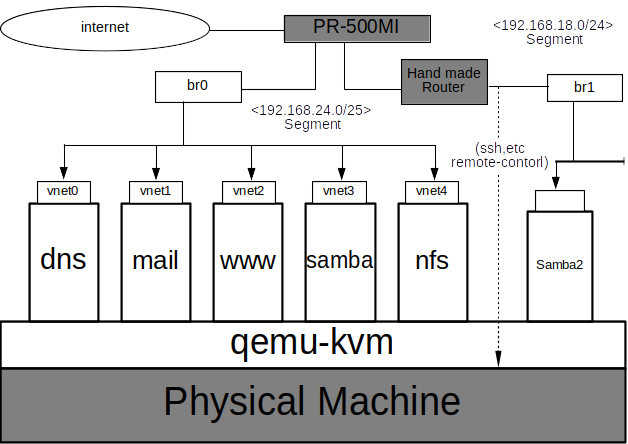
\includegraphics{image201803-kansai/external.png}
\caption{$B30ItMQ%M%C%H%o!<%/$N?^(B}
\end{figure*}
\clearpage

\subsubsection{$B30ItMQ%M%C%H%o!<%/$N@_Dj(B}
$B30ItMQ$N%M%C%H%o!<%/$G$N3F(BVM$B$N%M%C%H%o!<%/%G%P%$%9$N@_Dj$O!"Bh0l$K(Bvirt-manager$B$r;H$$2>A[%M%C%H%o!<%/$r@\B3$9$k2>A[(Bbridge$B$r:n@.$7$^$9!#<!$K(BVM$B$N%M%C%H%o!<%/%$%s%?!<%U%'%$%9$O!"(Bqemu$B$G%(%_%e%l!<%H$5$l$k(BTAP$B%G%P%$%9$r:n@.$7$F!"C1=c$KF~=PNO$r@\B3$9$k!V(Btap$B!W$r:n$j$^$9!#$3$N(Btap$B$O5<;wE*$J(Bethernet$B%G%P%$%9$G(BLinux$B%+!<%M%k$N5!G=$G$9!#$3$N2>A[E*$J(Bethernet$B%G%P%$%9$r!"F1$8$/(BLinux$B$N%+%M!<%k$N5!G=$G$"$k2>A[(Bbridge$B$G@\B3$9$k$3$G!"(BVM$B$O<B%G%P%$%9$d$[$+$N(BVM$B$H@\B3$9$k$3$H$,$G$-$^$9!#(B

$B$?$@$7!"(Bvirt-manager$B$G:n@.$9$k2>A[(Bbridge$B$O(Bdefault$B$G%5%V%M%C%H$r@_Dj$G$-$^$;$s!#$J$N$G!"(Binterfaces$B%U%!%$%k$rD>@\!"JT=8$7$F%5%V%M%C%H$r@_Dj$7$^$9!#$^$?!"(BHand made Router$B!"(BVM$B$N(BDNS$B$NN>J}$K(Bbind$B%Q%C%1!<%8$r%$%s%9%H!<%k$7!"30ItMQ%M%C%H%o!<%/$r9=C[$7$^$9!#(B

$B<!$K!"(BHand made Router$B$O%k!<%?$K$9$k$?$a$K!"(Biptables$B$H(Biptables-persisten$B$N%Q%C%1!<%8$r;H$$$^$9!#$^$?!"(B/etc/sysctl.conf$B$N(Bnet.ipv4.ip$B!2(Bforward=1$B$N%3%a%s%H$r30$7$F$*$-$^$9!#6qBNE*$K$O(B

\begin{itemize}
\item $B2>A[(Bbridge$B!"(BHand made Router$B$G$N%5%V%M%C%H$N@_Dj(B\\
VM$B$rAv$i$;$k<B5!$O(B qemu-kvm virt-manager$B$r%$%s%9%H!<%k$7$F@_Dj$7$^$9!#$=$7$FF15!$N(B/etc/network/interfaces$B$r0J2<$N$h$&$KD>@\!"JT=8$7$^$9!#(B
\begin{commandline}
# The loopback network interface
auto lo
iface lo inet loopback

# The primary network interface
allow-hotplug br0
iface br0 inet static
   address 192.168.24.108
   netmask 255.255.255.128
   gateway 192.168.24.1
   bridge$B!2(Bports enp9s0
   bridge$B!2(Bstp on
   bridge$B!2(Bfd 0.0
# This is an autoconfigured IPv6 interface
iface enp9s0 inet6 auto

# The secondary network interface
auto enx0022cf56e5ca
allow-hotplug enx0022cf56e5ca
iface enx0022cf56e5ca inet static
address 192.168.18.80
netmask 255.255.255.0
gateway 192.168.18.80
# This is an autoconfigured IPv6 interface
iface enx0022cf56e5ca inet6 auto
\end{commandline}
$B<!$K(BHand made Router$B$O%k!<%?$H$7$F5!G=$7!"(BVM$B$N%b%K%?!<$HJ]<i$b9T$$!"%$%s%?!<%M%C%H$+$i$NF~8}$K$b$7$^$9!#@_Dj$H$7$F$O(B /etc/network/interfaces$B$H(B/etc/iptables/rules.v4$B$r0J2<$NMM$K$7$^$9!#(B\\
--------interfaces--------
\begin{commandline}
# The loopback network interface
auto lo
iface lo inet loopback

# The primary network interface
auto enp2s1
allow-hotplug enp2s1
iface enp2s1 inet static
address 192.168.24.88
netmask 255.255.255.128
gateway 192.168.24.1

# This is an autoconfigured IPv6 interface
iface enp2s1 inet6 auto

# The secondary network interface
allow-hotplug ens32
iface ens32 inet static
address 192.168.18.1
netmask 255.255.255.0
gateway 192.168.18.1

# This is an autoconfigured IPv6 interface
iface ens32 inet6 auto
\end{commandline}
\clearpage
--------rules.v4--------
\begin{commandline}
# Generated by iptables-save v1.6.0 on Sat Nov 18 17:30:00 2017
*filter
:INPUT ACCEPT [0:0]
:FORWARD ACCEPT [0:0]
:OUTPUT ACCEPT [0:0]

-A INPUT -i lo -j ACCEPT
...(Omltted)...
-A INPUT -i enp2s1 -m state --state RELATED,ESTABLISHED -j ACCEPT
-A INPUT -i enp2s1 -j DROP
...(Omltted)...
-A FORWARD -o ens32 -j REJECT --reject-with icmp-port-unreachable
-A FORWARD -i enp2s1 -m state --state RELATED,ESTABLISHED -j ACCEPT
-A FORWARD -o ens32 -m state --state NEW,ESTABLISHED -j ACCEPT

-A FORWARD -i enp2s1 -j DROP
-A FORWARD -o ens32 -j DROP

-A OUTPUT -o lo -j ACCEPT
...(Omltted)...
-A OUTPUT -o ens32 -m state --state NEW,ESTABLISHED -j ACCEPT
-A OUTPUT -o ens32 -j DROP
COMMIT
# Completed on Sat Mar 25 17:12:38 2017

# Generated by iptables-save v1.6.0 on Sat Apr 29 10:00:07 2017
*mangle
:PREROUTING ACCEPT [0:0]
:INPUT ACCEPT [0:0]
:FORWARD ACCEPT [0:0]
:OUTPUT ACCEPT [0:0]
:POSTROUTING ACCEPT [0:0]
-A POSTROUTING -o ens32 -p udp -m udp --dport 68 -j CHECKSUM --checksum-fill
COMMIT
# Completed on Sat Aug 26 16:07:34 2017

# Generated by iptables-save v1.4.21 on Sat Aug 26 16:07:34 2017
*nat
:PREROUTING ACCEPT [0:0]
:INPUT ACCEPT [0:0]
:OUTPUT ACCEPT [0:0]
:POSTROUTING ACCEPT [0:0]

-A POSTROUTING -s 192.168.18.0/24 ! -d 192.168.18.0/24 -j SNAT --to-source 192.168.24.88
COMMIT
# Completed on Sat Nov 18 17:30:00 2017  
\end{commandline}

\clearpage

\item bind$B$N3F%9%F!<%?%9$r;H$C$?30ItMQ%M%C%H%o!<%/$N@_Dj(B\\
$B!!(BVM$B$N(BDNS$B!"(BHand Made Router$B$K%$%s%9%H!<%k$9$k(Bbind$B%Q%C%1!<%8$N(Bnamed.conf$B$N@_DjJ}K!$O2<?^$NDL$j!#35MW$H$7$F$O@_Dj%U%!%$%k$N(Bnamed.conf$B$K(Binclude$B%9%F!<%a%s%H$r;H$$!"(Bacl$B%9%F!<%H%a%s%H!"(Boptions$B%9%F!<%H%a%s%H$N@_Dj%U%!%$%k$rA^F~$7$^$9!#F1MM$K(Bview$B%9%F!<%H%a%s%H$G!">r7oIU$1%U%!%$%k$K$h$kF0:n$rDj5A$7!"(Binclude$B%9%F!<%H%a%s%H$G>r7o%U%!%$%k$rA^F~$7$^$9!#(B
%$B?^7A$NA^F~(B
\begin{figure*}[!h]
\centering
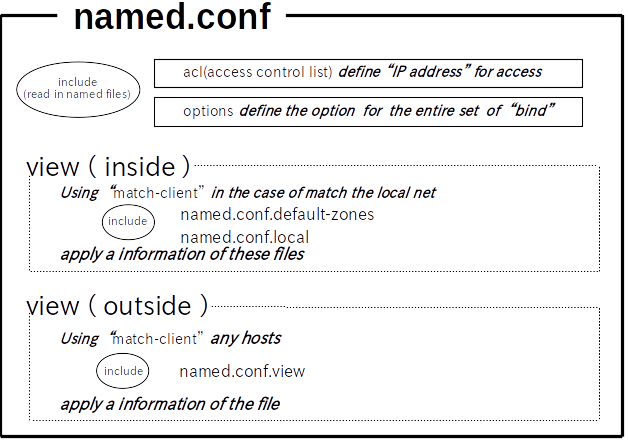
\includegraphics{image201803-kansai/named_conf.png}
\caption{named.conf$B$N?^(B}
\end{figure*}

$B0J2<!"3F@_Dj%U%!%$%k$N>\:Y$G$9!#(B
\clearpage

\item named.conf$B!J(Bbind$B$N@_Dj%U%!%$%k!K(B
\begin{commandline}
// This is the primary configuration file for the BIND DNS server named.
//
// Please read /usr/share/doc/bind9/README.Debian.gz for information on the 
// structure of BIND configuration files in Debian, *BEFORE* you customize 
// this configuration file.
//
// If you are just adding zones, please do that in /etc/bind/named.conf.local

include "/etc/bind/named.conf.acl";
include "/etc/bind/named.conf.options";

view "internal"{
	match-clients { localnet; };
	recursion yes;

include "/etc/bind/named.conf.local";
include "/etc/bind/named.conf.default-zones";

};

view "external" {
	match-clients { any; };
	recursion no;

include "/etc/bind/named.conf.view";

};    
\end{commandline}
$B3F%9%F!<%H%a%s%H$4$H$N@_Dj%U%!%$%k$O0J2<$N$h$&$K$J$j$^$9!#(B\\

\item acl$B%9%F!<%H%a%s%H!J%"%/%;%9$9$k%M%C%H%o!<%/$N(BIP$B%"%I%l%9$N@_Dj%U%!%$%k!K(B
\begin{commandline}
acl localnet{ 
	192.168.24.0/25;
	192.168.24.128/26;
	192.168.24.192/26;
	192.168.18.0/24; 
	127.0.0.1; 
};
\end{commandline}

\item options$B%9%F!<%H%a%s%H!J%*%W%7%g%s$G(Bbind$BA4BN$NF0:n$r@_Dj$9$k!K(B
\begin{commandline}
options {
	directory "/var/cache/bind";

	// If there is a firewall between you and nameservers you want
	// to talk to, you may need to fix the firewall to allow multiple
	// ports to talk.  See http://www.kb.cert.org/vuls/id/800113

	// If your ISP provided one or more IP addresses for stable 
	// nameservers, you probably want to use them as forwarders.  
	// Uncomment the following block, and insert the addresses replacing 
	// the all-0's placeholder.

	forwarders {
	 	8.8.8.8; 8.8.4.4;
	};

	//========================================================================
	// If BIND logs error messages about the root key being expired,
	// you will need to update your keys.  See https://www.isc.org/bind-keys
	//========================================================================
	dnssec-validation auto;
	allow-query { any; };
        allow-transfer{ 
		localnet;
		8.8.8.8;
		8.8.4.4; 
	};
	version "no version";
	auth-nxdomain no;    # conform to RFC1035
	listen-on-v6 { any; };
};
\end{commandline}
\clearpage

\item viwe$B%9%F!<%H%a%s%H!JFbIt!K(B\\
  match-client$B$r;H$$%m!<%+%k%M%C%H$K0J2<$N@_Dj%U%!%$%k$rE,MQ$9$k!#(B\\
--- named.conf.default-zone ---
\begin{commandline}
// prime the server with knowledge of the root servers
zone "." {
	type hint;
	file "/etc/bind/db.root";
};

// be authoritative for the localhost forward and reverse zones, and for
// broadcast zones as per RFC 1912

zone "localhost" {
	type master;
	file "/etc/bind/db.local";
};

zone "127.in-addr.arpa" {
	type master;
	file "/etc/bind/db.127";
};

zone "0.in-addr.arpa" {
	type master;
	file "/etc/bind/db.0";
};

zone "255.in-addr.arpa" {
	type master;
	file "/etc/bind/db.255";
};
\end{commandline}
zone$B%9%F!<%H%a%s%H!J%[%9%HL>$H(BIP$B%"%I%l%9$NBP1~4X78$N%j%9%H$rDj5A$9$k!K$G;H$o$l$F$$$k$3$l$i$N%U%!%$%k$O(Bdefault$B$G(Bbind$B%U%)%k%@$K4^$^$l$F$$$^$9!#(B\\
--- named.conf.local ---
\begin{commandline}
//
// Do any local configuration here
//
zone "kinsen.gr.jp" {
	type master;
	file "/etc/bind/db.in-kinsen.gr.jp";
};
zone "24.168.192.in-addr.arpa" {
	type master;
	file "/etc/bind/db.192.168.24";
};
zone "18.168.192.in-addr.arpa" {
	type master;
	file "/etc/bind/db.192.168.18";
};
// Consider adding the 1918 zones here, if they are not used in your
// organization
//include "/etc/bind/zones.rfc1918";
\end{commandline}
$B0J>e$N%U%!%$%k$O0J2<$NDL$j$G$9!#(B
\clearpage

--- db.in-kinsen.gr.jp ---
\begin{commandline}
;
; BIND data file for kinsen.gr.jp
;
$TTL	86400
@	IN     SOA      bandai.kinsen.gr.jp. root.bandai.kinsen.gr.jp. (
		              1         ; Serial
			   1800         ; Refresh
			    900         ; Retry
			 604800         ; Expire
			   1200 )       ; Negative Cache TTL

		IN      NS      dns

; localhost
localhost       IN      A       127.0.0.1
localhost       IN      AAAA    ::1

; Mail exchange
                IN      MX      0 mail.kinsen.gr.jp.
;
; Host entry
;
mizu0           IN      A       192.168.18.1
;               IN      AAAA    2001
mizu1           IN      A       192.168.18.2
;               IN      AAAA    2001
kamaba          IN      A       192.168.18.80
;               IN      AAAA    2001
noren           IN      A       192.168.24.108
;               IN      AAAA    2001
dns             IN      A       192.168.24.81
;               IN      AAAA    2001:
mail            IN      A       192.168.24.82
;               IN      AAAA    2001:
www             IN      A       192.168.24.83
;               IN      AAAA    2001:
karan           IN      A       192.168.24.84
;               IN      AAAA    2001:
datuiba         IN      A       192.168.24.85
;               IN      AAAA    2001:
bandai          IN      A       192.168.24.88
;               IN      AAAA    2001:
yubune          IN      A       192.168.24.18
;               IN      AAAA    2001:
;
; Alias
;www            IN      CNAME    noren
;
; Domain
@               IN      A       192.168.24.88
                IN      MX 0    mail
\end{commandline}
--- db.192.168.24 ---
\begin{commandline}
;
; BIND data file for 192.168.24 network
;
$TTL	86400
@         IN    SOA     bandai.kinsen.gr.jp. root.bandai.kinsen.gr.jp. (
		              1         ; Serial
			   1800         ; Refresh
			    900         ; Retry
			 604800         ; Expire
			   1200 )       ; Negative Cache TTL

                IN      NS      dns
;
; Host entry
;
108             IN      PTR     noren.kinsen.gr.jp.
81              IN      PTR     dns.kinsen.gr.jp.
82              IN      PTR     mail.kinsen.gr.jp.
83              IN      PTR     www.kinsen.gr.jp.
84              IN      PTR     karan.kinsen.gr.jp.
85              IN      PTR     datuiba.kinsen.gr.jp.
88              IN      PTR     bandai.kinsen.gr.jp.
18              IN      PTR     yubune.kinsen.gr.jp.
\end{commandline}
\clearpage

\item view$B%9%F!<%H%a%s%H(B($B30It(B)\\
  match-client$B$r;H$$$9$Y$F$N30It(Bhost$B$K(Bnamed.conf.view$B%U%!%$%k$rE,MQ$9$k!#(B\\
--- named.conf.view ---
\begin{commandline}
zone "." {
	type hint;
	file "/etc/bind/db.root";
};
zone "kinsen.gr.jp"{
	type master;
	file "/etc/bind/db.out-kinsen.gr.jp";
};
zone "158.141.203.in-addr.arpa"{
	type master;
	file "/etc/bind/db.203.141.158";
};    
\end{commandline}
db.root$B%U%!%$%k$O(Bdefault$B$G(Bbind$B%U%)%k%@$K$"$j$^$9!#(Bout-kinsen.gr.jp$B!"(Bdb.203.141.158$B$K$D$$$F$O0J2<$NDL$j!#(B\\
--- out-kinsen.gr.jp ---
\begin{commandline}
;
; BIND data file for kinsen.gr.jp
;
$TTL	86400
@        IN      SOA    bandai.kinsen.gr.jp. root.bandai.kinsen.gr.jp. (
                              1         ; Serial
			   1800         ; Refresh
			    900         ; Retry
			 604800         ; Expire
			   1200 )       ; Negative Cache TTL
                         $B!!!!!!!!!!!!!!!!!!!!(B
                IN$B!!!!!!(BNS       dns

; localhost
localhost       IN      A       127.0.0.1
localhost       IN      AAAA    ::1

; Mail exchange
                IN      MX      0 mail.kinsen.gr.jp.
;
; Host entry
;
noren           IN      A       203.141.158.41
;               IN      AAAA    2001:
dns             IN      A       203.141.158.41
;               IN      AAAA    2001:
mail            IN      A       203.141.158.41
;               IN      AAAA    2001:
www             IN      A       203.141.158.41
;               IN      AAAA    2001:
karan           IN      A       203.141.158.41
;               IN      AAAA    2001:
datuiba         IN      A       203.141.158.41
;               IN      AAAA    2001:
bandai          IN      A       203.141.158.41
;               IN      AAAA    2001:
yubune          IN      A       203.141.158.41
;               IN      AAAA    2001:
;
; Domain
@               IN      A       203.141.158.41
                IN      MX 0    mail
\end{commandline}
\clearpage

--- db.203.141.58 ---
\begin{commandline}
;
; BIND data file for 203.141.158 network
;
$TTL    86400
@       IN      SOA     bandai.kinsen.gr.jp. root.bandai.kinsen.gr.jp. (
                              1         ; Serial
                           1800         ; Refresh
                            900         ; Retry
                         604800         ; Expire
                           1200 )       ; Negative Cache TTL

                  IN        NS      dns
;
; Host entry
;
41		IN	PTR	noren.kinsen.gr.jp.
41		IN	PTR	dns.kinsen.gr.jp.
41		IN	PTR	mail.kinsen.gr.jp.
41		IN	PTR	www.kinsen.gr.jp.
41		IN	PTR	karan.kinsen.gr.jp.
41		IN	PTR	datuiba.kinsen.gr.jp.
41		IN	PTR	bandai.kinsen.gr.jp.
41		IN	PTR	yubune.kinsen.gr.jp.
\end{commandline}
\end{itemize}

\subsection{$BFbItMQ%M%C%H%o!<%/(B}
\subsubsection{$BFbItMQ%M%C%H%o!<%/$N35MW(B}
$BFbItMQ%M%C%H%o!<%/$O<B5!(BPC$B$K2>A[%k!<%?$r:n$j!"(BWifi$B7PM3$G<B5!>e$GAv$k(BVM$B$r%W%i%$%Y!<%H%M%C%H$r(B3$B$KJ,$1$?$=$l$>$l$N%;%0%a%s%H!J(B192.168.24.0/25 192.168.24.128/26 1923168.24.192/26$B!K$K$D$J$.$^$9!#(B\\
$B35MW$O2<?^$NDL$j!#(B

%$B?^7A$NA^F~(B
\begin{figure*}[!h]
\centering
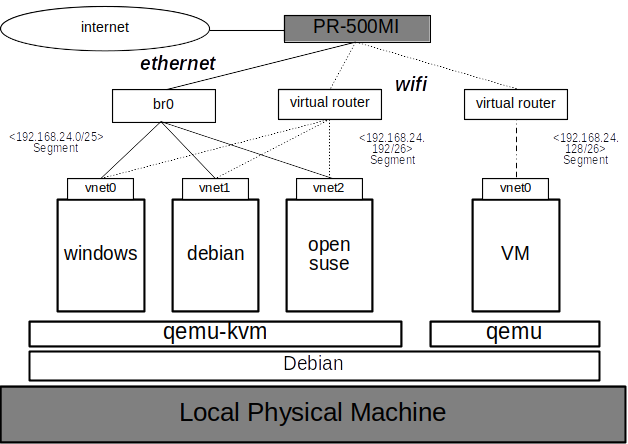
\includegraphics{image201803-kansai/internal.png}
\caption{$BFbItMQ%M%C%H%o!<%/$N?^(B}
\end{figure*}
\clearpage

\subsubsection{$BFbItMQ%M%C%H%o!<%/$N@_Dj(B}
$BFbItMQ%M%C%H%o!<%/$N@_Dj$O!"A0Ds$H$7$F(Bvirt-manager$B$N(BConnection Details$B$N(Bvirtual network$B$G2>A[%k!<%?$r:n$C$F$*$-$^$9!#$^$?!"<B5!(BPC$B$r%k!<%?$K$9$k;v$rA0Ds$K$7$F$$$^$9$N$G!"A0=R$N(BHand made Router$B$N$h$&$K!"(Binterfaces$B$H(Brules.v4$B$N%U%!%$%k$r0J2<$N$h$&$K@_Dj$7$^$9!#(B

--- interfaces ---
\begin{commandline}
# This file describes the network interfaces available on your system
# and how to activate them. For more information, see interfaces(5).

source /etc/network/interfaces.d/*

# The loopback network interface
auto lo
iface lo inet loopback

# The primary network interface
allow-hotplug wlp1s0
iface  wlp1s0 inet dhcp

# This is an autoconfigured IPv6 interface
iface wlp1s0 inet6 auto

# The primary network interface
allow-hotplug enx0022cf56e5ca
iface br0 inet static
   address 192.168.24.8
   netmask 255.255.255.128
   gateway 192.168.24.1
   bridge_ports enx0022cf56e5ca
   bridge_stp on
   bridge_fd 0.0
# This is an autoconfigured IPv6 interface
iface enx0022cf56e5ca inet6 auto
iface br0 inet6 auto
\end{commandline}
\clearpage

--- rules.v4 ---
\begin{commandline}
# Generated by iptables-save v1.6.0 on Sat Apr 29 10:00:07 2017
*filter
:INPUT ACCEPT [0:0]
:FORWARD ACCEPT [0:0]
:OUTPUT ACCEPT [0:0]
-A INPUT -i lo -j ACCEPT
-A INPUT -i enx0022cf56e5ca -j ACCEPT
-A INPUT -i br0 -j ACCEPT

-A INPUT -i wlp1s0 -p udp -m udp --dport 123 -j ACCEPT
-A INPUT -i wlp1s0 -p udp -m udp --dport 53 -j ACCEPT
-A INPUT -i wlp1s0 -p tcp -m tcp --dport 53 -j ACCEPT
-A INPUT -i wlp1s0 -p udp -m udp --dport 67:68 -j ACCEPT
-A INPUT -i wlp1s0 -p tcp -m tcp --dport 80 -j ACCEPT
-A INPUT -i wlp1s0 -p tcp -m tcp --dport 443 -j ACCEPT
-A INPUT -i wlp1s0 -p udp -m udp --dport 111 -j ACCEPT
-A INPUT -i wlp1s0 -p tcp -m tcp --dport 111 -j ACCEPT
-A INPUT -i wlp1s0 -p udp -m udp --dport 2049 -j ACCEPT
-A INPUT -i wlp1s0 -p tcp -m tcp --dport 2049 -j ACCEPT
-A INPUT -i wlp1s0 -p udp -m udp --dport 445 -j ACCEPT
-A INPUT -i wlp1s0 -p tcp -m tcp --dport 445 -j ACCEPT
-A INPUT -i wlp1s0 -p tcp -m tcp --dport 5900:6000 -j ACCEPT
-A INPUT -i wlp1s0 -p udp -m udp --dport 32800:32805 -j ACCEPT
-A INPUT -i wlp1s0 -p tcp -m tcp --dport 32800:32805 -j ACCEPT
-A INPUT -i wlp1s0 -m state --state RELATED,ESTABLISHED -j ACCEPT
-A INPUT -i wlp1s0 -j DROP


-A FORWARD -i wlp1s0 -p udp -m udp --dport 123 -j ACCEPT
-A FORWARD -o virbr1 -p udp -m udp --sport 123 -m state --state ESTABLISHED -j ACCEPT
-A FORWARD -i wlp1s0 -p udp -m udp --dport 53 -j ACCEPT
-A FORWARD -o virbr1 -p udp -m udp --sport 53 -m state --state ESTABLISHED -j ACCEPT
-A FORWARD -i wlp1s0 -p tcp -m tcp --dport 53 -j ACCEPT
-A FORWARD -o virbr1 -p tcp -m tcp --sport 53 -m state --state ESTABLISHED -j ACCEPT
-A FORWARD -i wlp1s0 -p udp -m udp --dport 67 -j ACCEPT
-A FORWARD -o virbr1 -p udp -m udp --sport 67 -m state --state ESTABLISHED -j ACCEPT
-A FORWARD -i wlp1s0 -p udp -m udp --dport 68 -j ACCEPT
-A FORWARD -o virbr1 -p udp -m udp --sport 68 -m state --state ESTABLISHED -j ACCEPT
-A FORWARD -i wlp1s0 -p tcp -m tcp --dport 80 -j ACCEPT
-A FORWARD -o virbr1 -p tcp -m tcp --sport 80 -m state --state ESTABLISHED -j ACCEPT
-A FORWARD -i wlp1s0 -p tcp -m tcp --dport 443 -j ACCEPT
-A FORWARD -o virbr1 -p tcp -m tcp --sport 443 -m state --state ESTABLISHED -j ACCEPT
-A FORWARD -i wlp1s0 -p udp -m udp --dport 445 -j ACCEPT
-A FORWARD -o virbr1 -p udp -m udp --sport 445 -m state --state ESTABLISHED -j ACCEPT
-A FORWARD -i wlp1s0 -p tcp -m tcp --dport 445 -j ACCEPT
-A FORWARD -o virbr1 -p tcp -m tcp --sport 445 -m state --state ESTABLISHED -j ACCEPT
-A FORWARD -i wlp1s0 -p tcp -m tcp --dport 5900:6000 -j ACCEPT
-A FORWARD -o virbr1 -p tcp -m tcp --sport 5900:6000 -m state --state ESTABLISHED -j ACCEPT
-A FORWARD -o virbr1 -j REJECT --reject-with icmp-port-unreachable
-A FORWARD -i wlp1s0 -m state --state RELATED,ESTABLISHED -j ACCEPT
-A FORWARD -o virbr1 -m state --state NEW,ESTABLISHED -j ACCEPT
-A FORWARD -i wlp1s0 -j DROP
-A FORWARD -o virbr1 -j DROP

-A OUTPUT -o lo -j ACCEPT
-A OUTPUT -o br0 -j ACCEPT

-A OUTPUT -o virbr1 -p udp -m udp --sport 123 -j ACCEPT
-A OUTPUT -o virbr1 -p udp -m udp --sport 53 -j ACCEPT
-A OUTPUT -o virbr1 -p tcp -m tcp --sport 53 -j ACCEPT
-A OUTPUT -o virbr1 -p udp -m udp --sport 67:68 -j ACCEPT
-A OUTPUT -o virbr1 -p tcp -m tcp --sport 80 -j ACCEPT
-A OUTPUT -o virbr1 -p tcp -m tcp --sport 443 -j ACCEPT
-A OUTPUT -o virbr1 -p udp -m udp --sport 111 -j ACCEPT
-A OUTPUT -o virbr1 -p tcp -m tcp --sport 111 -j ACCEPT
-A OUTPUT -o virbr1 -p udp -m udp --sport 2049 -j ACCEPT
-A OUTPUT -o virbr1 -p tcp -m tcp --sport 2049 -j ACCEPT
-A OUTPUT -o virbr1 -p udp -m udp --sport 445 -j ACCEPT
-A OUTPUT -o virbr1 -p tcp -m tcp --sport 445 -j ACCEPT
-A OUTPUT -o virbr1 -p tcp -m tcp --sport 5900:6000 -j ACCEPT
-A OUTPUT -o virbr1 -p udp -m udp --sport 32800:32805 -j ACCEPT
-A OUTPUT -o virbr1 -p tcp -m tcp --sport 32800:32805 -j ACCEPT
-A OUTPUT -o virbr1 -m state --state NEW,ESTABLISHED -j ACCEPT
-A OUTPUT -o virbr1 -j DROP
COMMIT

*mangle
:PREROUTING ACCEPT [0:0]
:INPUT ACCEPT [0:0]
:FORWARD ACCEPT [0:0]
:OUTPUT ACCEPT [0:0]
:POSTROUTING ACCEPT [0:0]
-A POSTROUTING -o virbr1 -p udp -m udp --dport 68 -j CHECKSUM --checksum-fill
COMMIT

*nat
:PREROUTING ACCEPT [0:0]
:INPUT ACCEPT [0:0]
:OUTPUT ACCEPT [0:0]
:POSTROUTING ACCEPT [0:0]
-A POSTROUTING -s 192.168.1.128/26 ! -d 192.168.1.128/26 -j MASQUERADE
-A POSTROUTING -s 192.168.1.192/26 ! -d 192.168.1.192/26 -j MASQUERADE
COMMIT
# Completed on Sat Jul 22 20:16:41 2017
\end{commandline}

\subsection{$B$^$H$a(B}
$B0J>e$,!"!V2f$,2H$N2>A[%M%C%H%o!<%/!W$NFbMF$G$9!#$?$@!"<B:]$N$H$3$mK\Mh$N%7%s%/%i%$%"%s%H$NL\E*$+$i$O%:%l$F$$$^$9!#:#8e$O(Bv6$B$N$X$NBP1~$d!"(BOS$B%5!<%P$J$k$b$NMQ0U$7$F!"99$J$k!IMxJX@-!I$rDI5a$9$k$D$b$j$G$9!#(B
\clearpage

%
% $B:};R$K$9$k$?$a$K!"(B4$B$NG\?t$K$9$kI,MW$,$"$k!#(B
% $B$=$N$?$a$ND4@0(B

\mbox{}\newpage
\mbox{}\newpage

\printindex
%\cleartooddpage

 \begin{minipage}[b]{0.2\hsize}
  \rotatebox{90}{\fontsize{80}{80} {\gt $B4X@>(B Debian $BJY6/2q(B} }
 \end{minipage}
 \begin{minipage}[b]{0.8\hsize}

 \vspace*{15cm}
 \rule{\hsize}{1mm}
 \vspace{2mm}
 
\includegraphics[width=2cm]{image200502/openlogo-nd.eps}
 \noindent \Large \bfseries{Debian $BJY6/2q;qNA(B}\\ \\
 \noindent \normalfont \debmtgyear{}$BG/(B\debmtgmonth{}$B7n(B\debmtgdate{}$BF|(B \hspace{5mm}  $B=iHGBh(B1$B:~H/9T(B\\
 \noindent \normalfont $B4X@>(B Debian $BJY6/2q(B $B!JJT=8!&0u:~!&H/9T!K(B\\
 \rule{\hsize}{1mm}
 \end{minipage}

\end{document}



